% Condensed manuscript. All claims and results come from paper/main.pdf.
\documentclass[conference,letterpaper]{IEEEtran}
\usepackage{amsmath}
\usepackage{graphicx}
\usepackage{microtype}
\usepackage{url}
\title{BC-GPTSwarm: Budget-Constrained Edge Optimization for Language-Agent Graphs}
\author{
\IEEEauthorblockN{Chirag Wattamwar}
\IEEEauthorblockA{202411029@iiitvadodara.ac.in}
\and
\IEEEauthorblockN{Kishan N Prasad}
\IEEEauthorblockA{202411054@iiitvadodara.ac.in}
\and
\IEEEauthorblockN{Kapil Kumar}
\IEEEauthorblockA{202411050@iiitvadodara.ac.in}
}
\begin{document}
\maketitle
\begin{abstract}
We implement BC-GPTSwarm, a modest primal--dual extension of GPTSwarm's language-agent edge optimizer for an explicit expected token budget. The method retains graph semantics and node roles while adding token telemetry, feasible-policy conditioning, corrected conditional gradients, and a learned non-negative multiplier. A reduced adversarial question-answering study uses a local half-billion-parameter model, one truthful and one adversarial agent, 24 held-out questions, and three seeds. The original accuracy-only baseline averages 0.250 accuracy and 251.1 tokens per question. Middle-budget BC-GPTSwarm averages 0.236 accuracy and 236.7 tokens: 5.8\% fewer tokens, but 4.0\% above target. The low target is missed by 28.8\%; only the high target has aggregate slack. An ablation with two truthful and two adversarial agents reaches 0.278 accuracy at 419.5 tokens. Broad uncertainty supports neither superiority nor equivalence. The contribution is an implemented constraint mechanism and a controlled diagnosis: feasibility conditioning works and dual pressure is observable, but tight-budget convergence is not established within twelve iterations.
\end{abstract}
\begin{IEEEkeywords}
language agents, graph optimization, token budgets, primal--dual learning
\end{IEEEkeywords}

\section{Introduction and Context}
GPTSwarm models operations as nodes, agents as directed graphs, and a swarm as a composite graph of agents~\cite{pmlr-v235-zhuge24a}. It optimizes inter-agent connectivity with policy gradients and separately improves node behavior through prompt updates. Its reported edge objective maximizes task utility, although sampled graphs may require different numbers of calls and tokens. Resource requirements are reported but do not enter that objective.

We ask whether GPTSwarm's stochastic edge policy can satisfy an explicit expected token budget while retaining task accuracy. A constraint specifies a target in resource units and can be assessed by budget violation. Our contribution is a versioned reproduction of the core adversarial MMLU edge optimizer, a feasible primal--dual extension, and controlled comparisons against accuracy-only and fixed-penalty alternatives.

Cost-aware multi-agent systems are already well studied. AgentPrune prunes communication, Optima balances effectiveness and token efficiency, and AgentSlimming compresses workflows through node pruning and cheaper model substitution~\cite{zhang2024agentprune,chen2024optima,chen2026agentslimming}. G-Designer and MasRouter construct or route collaboration more broadly~\cite{zhang2024gdesigner,yue2025masrouter}; AgentDropout removes agents dynamically, and Debate Only When Necessary triggers collaboration using confidence~\cite{wang2025agentdropout,eo2025debate}. We claim neither generic efficiency novelty nor priority over these approaches. This work changes optimization within a retained GPTSwarm candidate graph and emphasizes the completed results.

\section{Method}
\subsection{Inherited Graph and Baseline}
GPTSwarm defines an agent as a directed acyclic graph (DAG), $G=(N,E,F,o)$: nodes $N$, directed edges $E$, node routines $F$, and output node $o$. Nodes execute in topological order using the input and available predecessor information; a decision node aggregates terminal outputs. Edge sampling, black-box language-model execution, and external utility evaluation remain separate. The original edge objective is
\begin{equation}
 \max_\theta\ \mathrm{E}_{G\sim D_\theta}[u_\tau(G)].
\end{equation}
Each candidate edge has a sigmoid inclusion probability. Edges are sampled sequentially and rejected if they would create a cycle. REINFORCE estimates the policy gradient, and Adam updates the logits. The original system also supports prompt-level node optimization, which is outside our reproduction scope.

The adapter retains publication-era commit \texttt{1e1e5899d51bde690672417cf92aa4de7b210422}, candidate-edge order, one Bernoulli logit per edge, cycle rejection, majority vote, raw binary-accuracy utility, and Adam. The 1T1A graph has one truthful and one adversarial agent and four candidate edges: both inter-agent directions and each agent's edge to the decision node. Single-node agents always receive the original MMLU question. Inter-agent edges therefore primarily control scheduling and which answers reach the decision node.

Provider-independent responses, deterministic seeds, immutable data snapshots, and JSONL/CSV logging measure behavior without changing baseline reward. Provider errors, unparseable answers, and invalid decision input are retained and scored incorrect.

\subsection{Expected-Token Constraint}
Let $U(G,x)$ be task utility, $C(G,x)$ the sum of provider-reported input and output tokens across model calls, and $B>0$ the target. BC-GPTSwarm solves
\begin{align}
 \max_\theta\quad &\mathrm{E}_{x,G}[U(G,x)]\\
 \text{subject to}\quad &\mathrm{E}_{x,G}[C(G,x)]\leq B.
\end{align}
The normalized constraint is $\mathrm{E}[C/B-1]\leq0$, giving
\begin{equation}
 \mathcal L(\theta,\lambda)=
 \mathrm{E}[U-\lambda(C/B-1)],\quad\lambda\geq0.
\end{equation}
The fixed-penalty control instead maximizes $\mathrm{E}[U-\alpha C/B_{\mathrm{ref}}]$ with predeclared $\alpha$. It does not adapt its penalty to the requested target. Dollar cost and latency are logged but excluded from the token constraint.

\subsection{Feasible Policy and Updates}
A disconnected or zero-call graph is not a valid budget solution. BC-GPTSwarm conditions on event $F$: at least one agent has an edge to the decision node. Because that node is a sink, these edges cannot create cycles. For their candidate set $E_D$,
\begin{align}
 q_\theta=P_\theta(F)&=1-\prod_{e\in E_D}(1-p_e),\\
 \log p_\theta(G\mid F)&=\log p_\theta(G)-\log q_\theta.
\end{align}
Rejection sampling enforces $F$. Subtracting $\log q_\theta$ is essential: otherwise samples come from the conditional distribution while the score-function gradient uses the wrong distribution.

For a batch of $M$ executions, set $A_i=U_i-\bar U$ and $s_i=A_i-\lambda(C_i/B-1)$. The implementation applies Adam to
\begin{equation}
 -\frac{1}{M}\sum_{i=1}^M s_i\log p_\theta(G_i\mid F)
\end{equation}
and performs the projected dual update
\begin{equation}
 \lambda\leftarrow[\lambda+\eta_\lambda(\bar C/B-1)]_+.
\end{equation}
Above-budget batches increase the penalty. The task evaluator and resource meter both inform the edge update; only measured cost drives the dual update. Node routines, prompts, decision rules, and cycle rejection remain baseline components.

The runner measures a valid truthful direct-path cost floor on the optimization split and rejects lower budgets. Model settings, prompts, candidate edges, and targets are frozen before optimization. After the fixed allowance, evaluation draws one graph per held-out example from the frozen feasible policy using a recorded seed. Thresholded export is available but is not used to estimate the proposed method's expected constraint. Feasible-accuracy, fixed-penalty, and constrained conditions share validity rules and optimization-call allowance; the publication-style original is kept separately to expose conditioning effects.

\begin{table*}[t]
\centering\small
\caption{Controlled local-model comparison: mean $\pm$ sample SD over three seeds. Original is the local publication-style accuracy-only reproduction. Comparator violations use the middle target. Compliance is the fraction of queries at or below the target.}
\label{tab:main}
\begin{tabular}{lrrrr}
\hline
Condition & Accuracy & Tokens/query & Norm.\ violation & Compliance\\
\hline
Original & $0.250\pm0.110$ & $251.1\pm90.4$ & $+0.104$ & 0.46\\
Feasible accuracy & $0.222\pm0.105$ & $239.6\pm19.6$ & $+0.053$ & 0.53\\
Fixed penalty & $0.208\pm0.083$ & $230.4\pm21.3$ & $+0.013$ & 0.54\\
BC 0.50 & $0.208\pm0.110$ & $232.3\pm31.9$ & $+0.288$ & 0.38\\
BC 0.75 & $0.236\pm0.105$ & $236.7\pm29.8$ & $+0.040$ & 0.50\\
BC 1.00 & $0.208\pm0.083$ & $238.9\pm18.5$ & $-0.212$ & 0.75\\
\hline
\end{tabular}
\end{table*}

\section{Experimental Protocol}
We use the \texttt{all} configuration of \texttt{cais/mmlu} at immutable revision \texttt{c30699e8356da336a370243923dbaf21066bb9fe}, with 24 subject-diverse development examples for optimization and 24 disjoint validation examples for evaluation. Seeded SHA-256 subject ordering and committed snapshots record source indices, identifiers, and checksums.

The local provider is \texttt{qwen2.5:0.5b} through Ollama 0.17.1, at temperature zero, a four-token output cap, and model seed 20260918. Runs use Python 3.10.9, CPU-only PyTorch 2.8.0, a 16-logical-core Intel system, and approximately 16.9~GB RAM. Response caching is disabled. Raw responses, parsed answers, graph masks, token counts, latency, failures, gradients, and learned probabilities are logged.

All real-model conditions use seeds 11, 22, and 33; twelve iterations; batch size four; and primal learning rate 0.1. BC-GPTSwarm uses dual rate 0.2 and initial $\lambda=0$. The published MMLU setting used 200 iterations and 153 validation questions. Our reduced local setting is a behavioral reproduction and is not numerically comparable to the original GPT-4 Turbo-era endpoint.

The baseline tier compares direct, full, random ($p_e=0.5$), and accuracy-only optimized graphs. The controlled tier compares original accuracy-only, feasibility-matched accuracy-only, fixed penalty $\alpha=0.25$, and BC-GPTSwarm at budget ratios 0.50, 0.75, and 1.00 of the full-graph mean, 303.3 tokens/question. Operational targets are at least 105\% of the measured direct-path mean. With the new floor of 171.8 tokens, the low target becomes 180.4 rather than 151.6.

Primary outcomes are accuracy, mean tokens, normalized violation $\mathrm{E}[C/B-1]$, absolute budget error, and per-query compliance. One-factor middle-budget ablations change utility centering, dual rate (0.05 or 0.50), or graph scale (2T2A, sixteen candidate edges). Controlled condition order rotates by seed; all runs are retained.

The optimizer seed is the independent unit for learned-policy inference: three paired observations. We report sample standard deviations, exploratory 95\% Student-$t$ intervals with two degrees of freedom, and exact two-sided sign-flip tests. With three pairs the minimum attainable exact $p$ is 0.25. Secondary analysis uses exact McNemar testing on 72 matched seed--question outcomes and 20,000 bootstrap resamples of the 24 question clusters with fitted policies fixed. These outcomes are not independent optimizer replications; ablations are exploratory.
\section{Results}
\subsection{Validation and Baseline}
Fourteen offline tests pass, covering baseline behavior, DAG validity, parsing and data loading, conditional sampling and finite gradients, dual projection, cost sensitivity, fixed-dual controls, and paired statistical procedures. Mock and local-model smoke tiers complete without structural failures. The deterministic mock uses 117.6 mean tokens against a 130-token target, but this is software validation, not real-model research evidence.

The local baseline reproduction gives accuracies of 0.167 for direct answer, 0.264 for full connectivity, and 0.250 for both random and optimized graphs. Optimized graphs consume 6,027 tokens over 24 questions: 17.2\% fewer than full graphs but 35.0\% more than random graphs. Random graphs average 4.7 disconnected failures, so apparent savings partly reflect invalid execution.



\begin{figure*}[t]
\centering
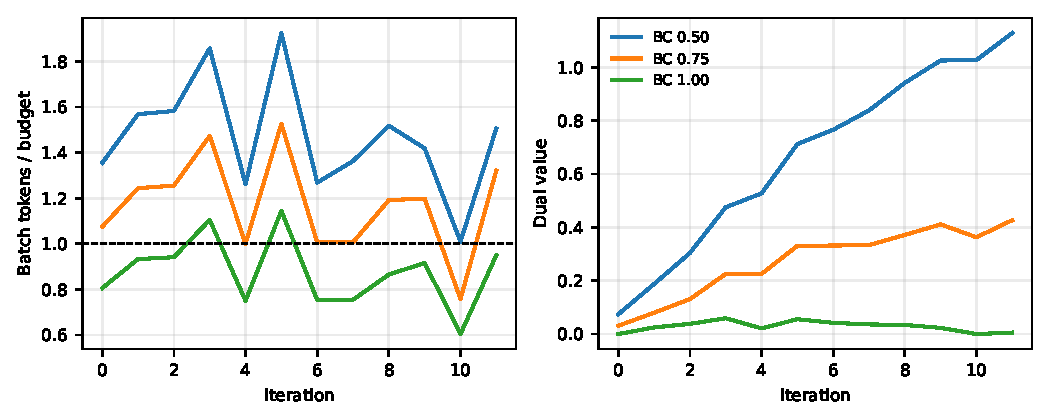
\includegraphics[width=0.9\textwidth]{../results/figures/optimization_stability.pdf}
\caption{Mean normalized training-batch cost and dual trajectories over three seeds. The dashed line marks the expected-budget boundary. Tight-budget penalties increase, but final training-batch costs remain above target.}
\label{fig:stability}
\end{figure*}

\begin{table*}[t]
\centering\small
\caption{Focal analysis: middle-budget BC minus original. Seed-level intervals use Student-$t$ with two degrees of freedom. The item-level interval is a fixed-seed question-cluster bootstrap; its test is exact McNemar.}
\label{tab:stats}
\begin{tabular}{lclrr}
\hline
Outcome & Unit ($n$) & Effect & 95\% CI & Exact $p$\\
\hline
Accuracy & seed (3) & $-1.39$ pp & $[-13.34,+10.56]$ & 1.000\\
Tokens/question & seed (3) & $-14.4$ tokens & $[-236.7,+207.8]$ & 0.750\\
Budget violation vs.\ zero & seed (3) & $+4.05\%$ & $[-28.52,+36.62]$ & 0.750\\
Accuracy (secondary) & seed--question (72) & $-1.39$ pp & $[-5.56,+2.78]$ & 1.000\\
\hline
\end{tabular}
\end{table*}

\subsection{Main Comparison}
\begin{figure}[t]
\centering
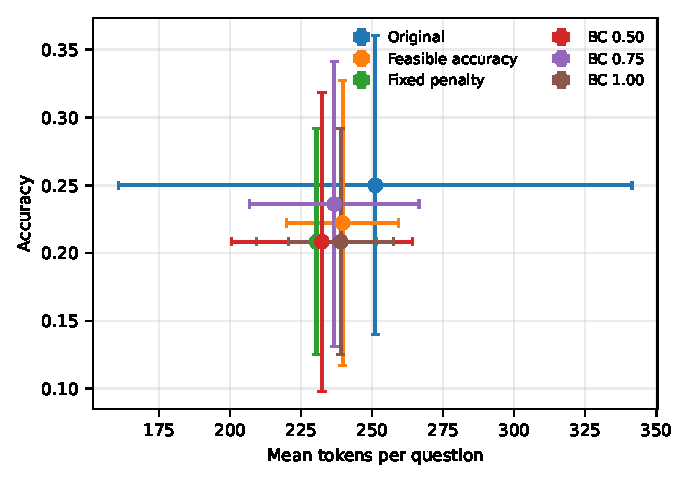
\includegraphics[width=\columnwidth]{../results/figures/main_accuracy_tokens.pdf}
\caption{Accuracy--token operating points for the controlled comparison. Error bars are sample standard deviations over three seeds.}
\label{fig:operating-points}
\end{figure}
Table~\ref{tab:main} summarizes eighteen controlled runs. Original accuracy-only optimization has the highest main-study mean accuracy, 0.250. Middle-budget BC-GPTSwarm reaches 0.236 at 236.7 rather than 251.1 tokens/question: a descriptive 5.8\% token reduction and a $-0.014$ accuracy difference. It nevertheless exceeds its expected target by 4.0\%. These observations do not establish an accuracy improvement or successful tight-budget enforcement.

Low-budget BC-GPTSwarm exceeds even its raised 180.4-token target by 28.8\%. High-budget BC-GPTSwarm averages 238.9 against a 303.3-token target, the only constrained setting with clear aggregate slack. Per-query compliance rises from 0.38 to 0.50 to 0.75 as targets loosen. Feasible accuracy-only and fixed-penalty controls average 0.222 and 0.208 accuracy; the latter uses 230.4 tokens, slightly fewer than default BC-GPTSwarm. All controlled main and ablation runs have zero provider errors, unparseable final answers, and disconnected graphs.

Observed cost changes little across budgets: 232.3 to 238.9 tokens while targets move from 180.4 to 303.3 (Fig.~\ref{fig:budget}). Feasible accuracy-only also lowers cost relative to the publication-style thresholded original. Savings against that original therefore do not isolate the learned dual mechanism; some come from feasible-policy evaluation.

\begin{figure}[t]
\centering
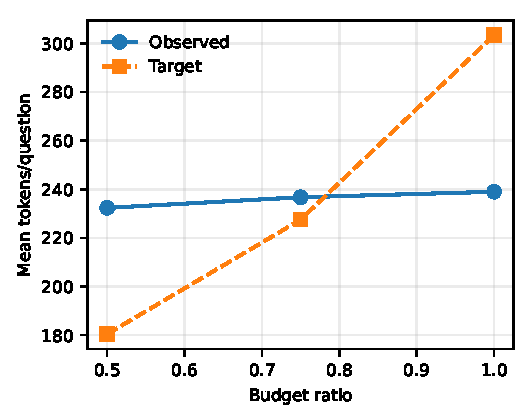
\includegraphics[width=0.9\columnwidth]{short_budget_response.pdf}
\caption{Token-budget response from the completed study (cost panel of the original budget-response figure). Observed mean cost varies weakly with the requested target.}
\label{fig:budget}
\end{figure}

\subsection{Mechanism Ablations}
\begin{table}[t]
\centering\small
\setlength{\tabcolsep}{3pt}
\caption{Middle-budget ablations: means over three seeds.}
\label{tab:ablation}
\begin{tabular}{lrrr}
\hline
Variant & Accuracy & Tokens & Violation\\
\hline
Centered / 1T1A & 0.236 & 236.7 & $+0.040$\\
Raw utility & 0.250 & 232.4 & $+0.022$\\
Dual rate 0.05 & 0.222 & 233.6 & $+0.027$\\
Dual rate 0.20 & 0.236 & 236.7 & $+0.040$\\
Dual rate 0.50 & 0.222 & 229.6 & $+0.009$\\
2T2A graph & 0.278 & 419.5 & $+0.844$\\
\hline
\end{tabular}
\end{table}
Raw utility matches the original mean accuracy, 0.250, with 232.4 tokens, but has accuracy SD 0.150. No tested dual rate has a stable accuracy advantage (Table~\ref{tab:ablation}). The 2T2A graph raises mean accuracy to 0.278 but costs 419.5 tokens and violates the middle target by 84.4\%. More agents increase both accuracy and resource use; this is not a useful constrained solution.

Final mean $\lambda$ values at ratios 0.50/0.75/1.00 are 1.129/0.427/0.005: tighter budgets correctly induce larger penalties. However, final training-batch cost ratios remain 1.506/1.321/0.950. The intended dual response is observable, but twelve iterations do not establish low- or middle-budget convergence.



Fig.~\ref{fig:operating-points} shows why accuracy and cost must be interpreted jointly: differences in the observed mean operating points are accompanied by substantial seed variation. Main-condition accuracy standard deviations range from 0.083 to 0.110. Fig.~\ref{fig:stability} separates a mechanically correct dual response from convergence: increasing the multiplier does not by itself establish budget feasibility.

\subsection{Uncertainty and Paired Outcomes}

All focal seed-level confidence intervals include zero (Table~\ref{tab:stats}). The paired accuracy effect is $-1.39$ percentage points, and the token effect is $-14.4$ tokens/question ($-5.75\%$ relative to the baseline mean). Broad intervals permit effects in both directions. Mean middle-budget violation is $+4.05\%$, and two of three seed means exceed the target. A non-significant test against zero violation is not evidence of compliance or equivalence: no equivalence margin was declared.

Of 72 paired seed--question outcomes, both methods are correct in fifteen, both wrong in fifty-two, the original alone correct in three, and BC-GPTSwarm alone correct in two. Exact McNemar $p=1.000$; the matched odds ratio is 0.667 (95\% exact confidence interval $[0.056,5.820]$). Thus feasible sampling removes structural failures, while ordinary task errors from the small model dominate. The secondary item-level analysis cannot replace independent optimizer replications.

\section{Discussion and Limitations}
The central result is negative but informative. BC-GPTSwarm makes expected resource constraints measurable, prevents invalid zero-call solutions, and exhibits dual pressure in the correct direction. The completed study does not support the performance hypothesis: mean accuracy falls at the middle target, low and middle expected budgets remain unmet, and uncertainty prevents superiority or equivalence claims.

The controls separate these observations from a generic efficiency claim. Feasible accuracy-only optimization already reduces cost; a fixed penalty consumes slightly fewer tokens than default BC-GPTSwarm but has lower mean accuracy; raw utility gives a favorable mean point with larger variance. The larger graph improves mean accuracy at substantially greater cost. None provides a stable ranking under three seeds.

The evidence applies only to the declared reduced setting: a 0.5B model, 24 held-out questions, 1T1A graph, and twelve iterations. We cannot access the original 2024 endpoint, and we do not reproduce GPTSwarm's tool-use or node-optimization experiments. In the single-node MMLU path, all agents receive the question, limiting graph-dependent cooperation. Discrete graphs and binary rewards make primal--dual learning difficult, particularly with weak task performance.

An expected-token budget is not a per-query cap. Tokens imperfectly proxy monetary cost, latency, or energy. Baseline conditions run in fixed order, so warm-up confounds cross-method latency; local CPU load also affects wall time. A retained 2,109-second fixed-penalty optimization outlier further limits timing conclusions. We therefore make no independent latency success claim.

Three independent seeds produce coarse exact tests and broad intervals. Questions repeat across policies; the 72 matched outcomes are not 72 independent optimizer runs. No confirmatory ablation family or equivalence margin was preregistered. Synthetic smoke compliance validates software behavior only and cannot establish real-model efficacy.

\section{Conclusion and Future Work}
BC-GPTSwarm is an implemented feasible primal--dual extension of GPTSwarm for an explicit expected token budget. At the middle target, it uses 5.8\% fewer mean tokens than the original local baseline, but accuracy is 0.236 versus 0.250 and cost remains 4.0\% above target. The low target is also missed; only the high target has aggregate slack. The supported contribution is implementation and constraint diagnosis, not improved accuracy or established tight-budget control.

Future work should predeclare a longer optimization allowance and evaluate a stronger model or a task with more graph-dependent cooperation. These would be new experiments, not post-hoc repairs to the current results. The present evidence identifies convergence as the unresolved bottleneck.

% Start the reference list in the next column to balance the final page.
\newpage
\bibliographystyle{IEEEtran}
\bibliography{references}
\end{document}
